\chapter{Scenarii de utilizare}

În mod natural, persoanele dintr-o facultate utilizează aplicația \thesistitle în scopuri diferite în funcție de tipul lor. Fiecare este întâmpinat de pagina principală \textbf{Matching} care prezintă repartizarea tezelor de licență studenților în funcție de preferințele lor. Însă odată autentificat, interfața este adaptată nevoilor specifice utilizaotrului.

Un student poate vizualiza lista tuturor profesorilor și poate accesa propunerile unui anumit profesor. Acesta are opțiunea de a adăuga anumite proiecte sau tematici în lista proprie de preferințe, dacă nu au fost încă convenite în acorduri profesor-student. Preferințele urmează a fi ordonate în funcție de rating.

Un profesor care este are administrator, după autentificare, poate adăuga un cont pentru un nou student. Ulterior, profesorul poate încheia un acord cu acest student asupra unui proiect, dacă studentul acceptă o astfel de înțelegere, oferindu-i astfel șansa acestuia de a nu mai participa în etapa de reaprtizare algoritmică, fiindu-i deja atribuită o lucrare convenită.

\begin{figure}[H]
	\centering
	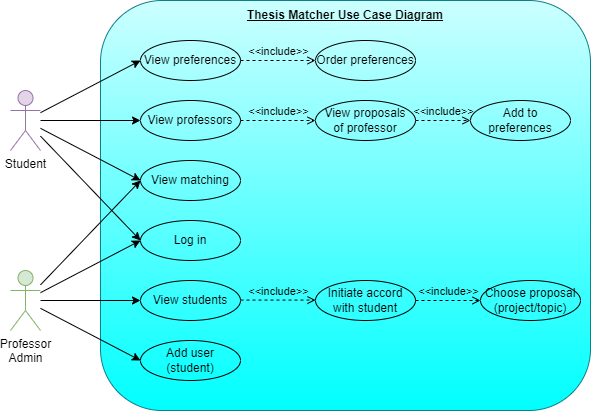
\includegraphics[width=1\textwidth, center]{use-case-diagram.png}
	\caption{Diagramă Use Case}
\end{figure}